% Scattering transform 

%%%% TO LATE CROP THE PDF AT THE CORRECT SIZE FOR PLOTING: %%%%
% pdfcrop --margins '-0 -0 -0 -422' scat_tree.pdf ../scat_tree_crop.pdf

% Tree for J = 4 M = 2 and L = 1
% Layer 0 : 1 node
% Layer 1 : 4 nodes
% Layer 2 : 6 nodes

\documentclass{article}
\usepackage{tikz}
\usetikzlibrary{arrows}

\tikzset{
  treenode/.style = {align=center, inner sep=0pt, text centered, font=\sffamily},
  % U node: empty black circle text abov
  arn_U/.style = {treenode, circle, black,minimum width=0.9cm, draw=black, minimum width=1.5em, font=\tiny}, % font=\sffamily\bfseries
  arn_S/.style = {treenode, circle, white, draw=black, fill=black, minimum width=1.5em, very thick},
  label_U/.style = {node distance=0mm, draw=white, fill=white!20}
  %   arn_x/.style = {treenode, rectangle, draw=black,
%     minimum width=0.5em, minimum height=0.5em}% arbre rouge noir, nil
}

\begin{document}
\hspace*{-35mm}%
	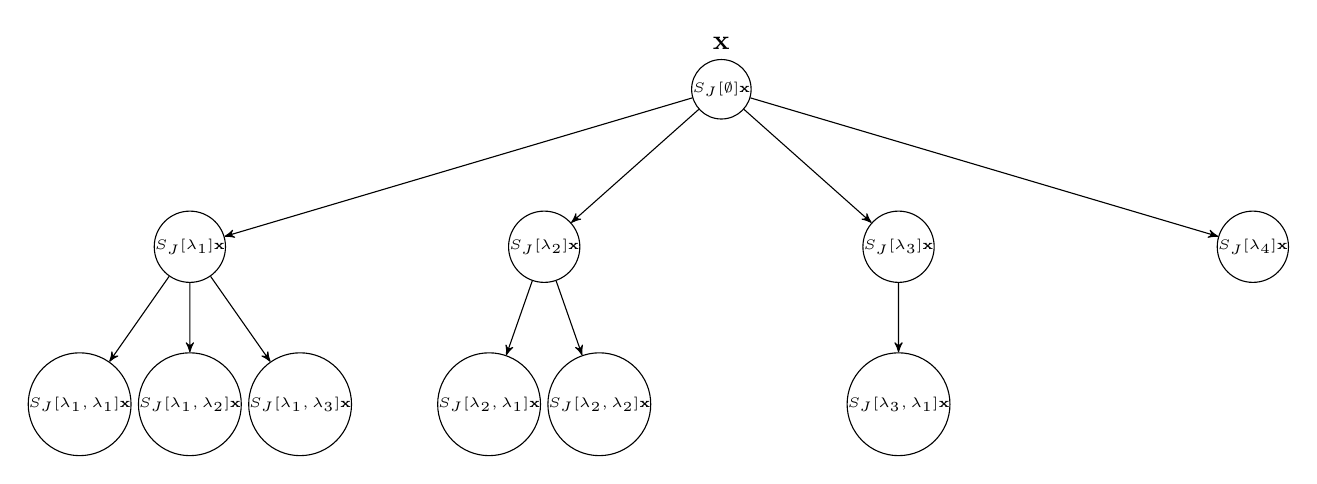
\begin{tikzpicture}[x=15cm,y=20cm,
		->,>=stealth',
		level 1/.style={sibling distance=45mm, level distance = 2cm},
    level 2/.style={sibling distance=12mm, level distance = 2cm}
    ] 
    % Root S node:
		\node [arn_U][label=above:{$\mathbf{x}$}][xshift=-10mm, yshift=+0mm] {$S_{J}[\emptyset]\mathbf{x}$}
			% S_{0} node:
%  			child{node [arn_S][xshift=+48mm, yshift=+18mm]
% 												[label={[draw=blue]left:{\color{blue}$S_{J}[\emptyset]\mathbf{x}=\mathbf{x} \ast \phi_{J}$}}]{}}
			% Layer 1 - S nodes:
			child{node [arn_U]{$S_{J}[\lambda_{1}]\mathbf{x}$}  
% 						% S_{1} node:
% 						child{node [arn_S][xshift=+5mm, yshift=+18mm]
% 															[label={[draw=blue]left:{\color{blue}$S_{J}[\lambda_{1}]\mathbf{x}$}}]{}}
						% Layer 2 - Propagation nodes:
						child{node [arn_U][xshift=-2mm, yshift=+0mm]{$S_{J}[\lambda_{1},\lambda_{1}]\mathbf{x}$}
% 							% S_{2} node:
% 							child{node [arn_S][xshift=-10mm, yshift=+18mm]
% 																[label={[draw=blue]left:{\color{blue}$S_{J}[\lambda_{1},\lambda_{2}]\mathbf{x}$}}]{}}
						}
						child{node [arn_U] {$S_{J}[\lambda_{1},\lambda_{2}]\mathbf{x}$}}
						child{node [arn_U][xshift=+2mm, yshift=+0mm]{$S_{J}[\lambda_{1},\lambda_{3}]\mathbf{x}$}}
							}
			child{node [arn_U]{$S_{J}[\lambda_{2}]\mathbf{x}$}
% 						% S_{1} node:
% 						child{node [arn_S][xshift=+0mm, yshift=+18mm]{}}
						% Layer 2 - Propagation nodes:
						child{node [arn_U][xshift=-1mm, yshift=+0mm] {$S_{J}[\lambda_{2},\lambda_{1}]\mathbf{x}$}}
						child{node [arn_U][xshift=+1mm, yshift=+0mm] {$S_{J}[\lambda_{2},\lambda_{2}]\mathbf{x}$}}
							}
			child{node [arn_U]{$S_{J}[\lambda_{3}]\mathbf{x}$}
% 						% S node:
% 						child{node [arn_S][xshift=-7mm, yshift=+18mm]{}}
						% Layer 2 - Propagation nodes:
						child{node [arn_U] {$S_{J}[\lambda_{3},\lambda_{1}]\mathbf{x}$}} %for a named pointer
							}
			child{node [arn_U]{$S_{J}[\lambda_{4}]\mathbf{x}$}
% 						% S_{2} node:
% 						child{node [arn_S][xshift=-13mm, yshift=+18mm]{}}
						% Layer 2 - Propagation nodes:
							}
		; 
	\end{tikzpicture}
\end{document}

% [label=left:{\color{blue}$S_{J}[\lambda_{1},\lambda_{2}]x$}]